\documentclass{beamer}

\usepackage{commun}
\usepackage{couleurs}
\usepackage{shortcuts}

\newcommand{\vdashrule}[1]{\tikz[remember picture]\draw[overlay](3.2,2.75)--+(0,-#1);}

\graphicspath{{images/}}

\usetheme{metropolis}

\title{MAN documentation et commande}
\subtitle{Architectures matérielles et système d'exploitation}
%\author{}
%\date{\today}

\begin{document}

\metroset{titleformat frame=smallcaps}

\maketitle

\nocite{*}

\section{Fiche pédagogique}

\begin{frame}{Présentation}
  \bi[<+- | alert@+>]
    \item L'activité se fait à la suite d'un cours d'introduction au système d'exploitation Unix.
    \item Problématique : comment accéder à la description et option des commandes sous Unix ?
    \item Plusieurs objectifs, à l'aide de la commande \texttt{man} :
    \be
      \item explorer les commandes de la console Unix ;
      \item exploiter l'outil <<\texttt{man}>> afin de connaître et comprendre les différentes options.
    \ee
  \ei
\end{frame}

\begin{frame}{Contexte}
  \uncover<+->{
    \bi[<+- | alert@+>]
      \item Durée : 2 heures
      \item Niveau : 1ère NSI
      \item Matériel nécessaire :
      \bi
        \item poste informatique sous Linux ;
        \item documents : sujet du TP et annexes.
      \ei
      \item Prérequis :
      \bi
        \item connaître la notion d'arborescence ;
        \item savoir se connecter dans un environnement Linux ;
        \item savoir accéder à une console ou un terminal.
      \ei
    \ei
  }
\end{frame}

\begin{frame}{Contexte}
\uncover<+->{
  \bi[<+- | alert@+>]
    \item Lien programme : Système d'exploitation (Architectures matérielles et système d'exploitation) ;
    \item Compétences travaillées :
    \bi
      \item utiliser les commandes de base en ligne de commande ;
      \item gérer une arborescence de fichiers et de dossiers ;
      \item gérer les droits et permissions d'accès aux fichiers.
    \ei
  \ei
}
\end{frame}

\begin{frame}{Déroulement de l'activité}
\uncover<+->{
  \be[<+- | alert@+>]
    \item Présentation de la nécessité de la commande \texttt{man}.
    \item Description de l'arborescence de fichiers et dossiers souhaitée.
    \item Mise en activité : connexion à la console et création de l'arborescence.
    \item Accès au manuel.
    \item Pour aller plus loin : <<\texttt{man} en français>> et autres commandes.
  \ee
}
\end{frame}

\section{La commande \texttt{man}}

\begin{frame}{Pourquoi ?}
  \uncover<+->{
    La commande \texttt{man} permet de visualiser le contenu de pages de documentation formatées pour celle-ci.\\
    Originellement, elle permet d'accéder aux manuels des commandes du shell Unix et à la description des fonctions du langage C.
  }
\end{frame}

\begin{frame}{Organisation ?}
  \uncover<+->{
    Il faut savoir que :
    \bi[<+- | alert@+>]
      \item la documentation n'est pas dans un seul et unique fichier ;
      \item elle se situe dans un répertoire du système (/usr/share/man sous Debian, par exemple) ;
      \item les pages du manuel sont organisées en \textbf{9 sections} :
      \be
        \item Programmes exécutables ou commandes de l'interpréteur de commandes (shell)
        \item Appels système (fonctions fournies par le noyau)
        \item Appels de bibliothèque (fonctions fournies par les bibliothèques des programmes)
        \item etc...
      \ee
%        \item Fichiers spéciaux (situés généralement dans /dev)
%        \item Formats des fichiers et conventions. Par exemple /etc/passwd
%        \item Jeux
%        \item Divers (y compris les macropaquets et les conventions), par exemple man(7), groff(7)
%        \item Commandes de gestion du système (généralement réservées au superutilisateur)
%        \item Sous-programmes du noyau [hors standard]
%      \ee
    \ei
  }
\end{frame}

\begin{frame}[fragile]{Comment ?}
  Il suffit de taper :
  \begin{minted}[]{shell}
    man [nom de la commande]
  \end{minted}
  
  \bi[<+- | alert@+>]
    \item\mintinline{shell}{man ls}\\
    Affiche la page de manuel de la commande \texttt{ls}.
    \item \mintinline{fish}{man passwd}\\
    Affiche la page de manuel de la commande \texttt{passwd}
    \item \mintinline{shell}{man 5 passwd}\\
    Affiche la page de manuel du fichier des mots de passe \texttt{passwd}
  \ei
\end{frame}

\begin{frame}[fragile]{À quoi ressemble une page de man ?}
  \uncover<+->{
    \begin{center}
      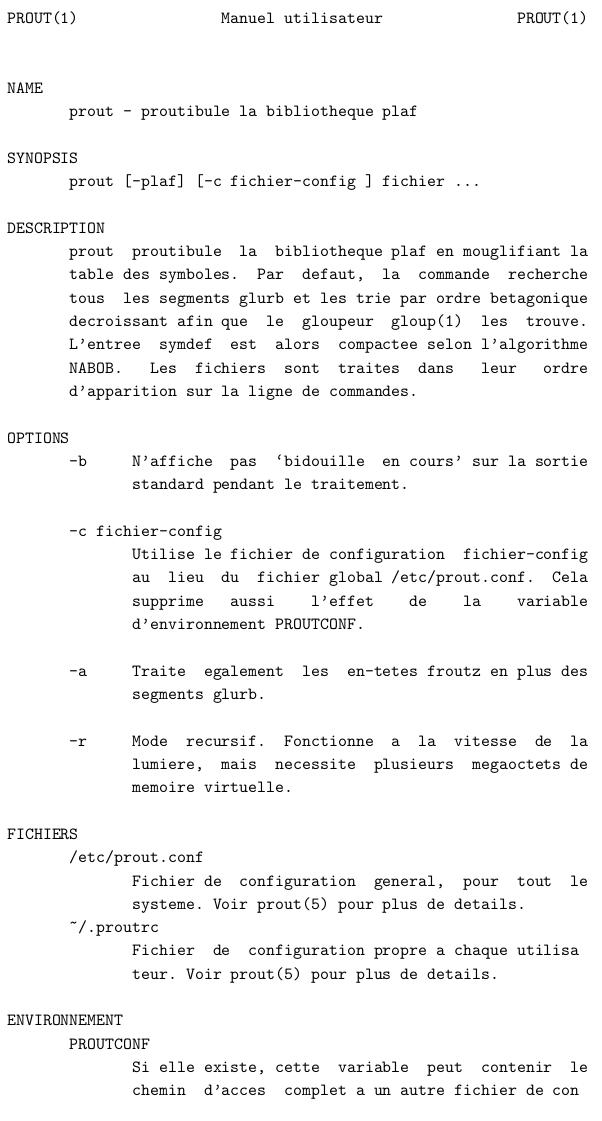
\includegraphics[scale=.3, trim={0 18cm 0 0}, clip]{page_de_man_exemple.png}
    \end{center}
    \begin{flushright}
      \footnotesize\textit{source : }\href{http://www.tldp.org/pub/Linux/docs/HOWTO/translations/fr/pdf/Man-Page.pdf}{www.tldp.org}
    \end{flushright}
  }
\end{frame}


\section{Activité}

\section*{Sommaire}

\begin{frame}{Sommaire}
  \tableofcontents
\end{frame}




\end{document}
